\chapter{Change of Basis and Similarity}
\label{ch:change-basis-similarity}

\section{Vectors Are Not Their Coordinate Lists}

The vector $(4,2)$ is a coordinate description in the standard basis of
$\R^2$. If we use a different basis, the same geometric vector has a different
coordinate list.

Let
\[
  b_1=\begin{bmatrix}1\\1\end{bmatrix},
  \qquad
  b_2=\begin{bmatrix}1\\-1\end{bmatrix}.
\]
To write
\[
  v=\begin{bmatrix}4\\2\end{bmatrix}
\]
in this basis, solve
\[
  c_1b_1+c_2b_2=v.
\]
That is
\[
  \begin{bmatrix}
  1&1\\
  1&-1
  \end{bmatrix}
  \begin{bmatrix}c_1\\c_2\end{bmatrix}
  =
  \begin{bmatrix}4\\2\end{bmatrix}.
\]
The solution is
\[
  c_1=3,\qquad c_2=1,
\]
so the same vector has $B$-coordinates
\[
  [v]_B=\begin{bmatrix}3\\1\end{bmatrix}.
\]

\begin{warningbox}
Coordinates depend on a basis. The vector does not. Many mistakes in change
of basis come from treating a coordinate list as if it were the object itself.
\end{warningbox}

\section{Coordinate Maps}

\begin{definition}[Basis matrix]
Let $B=(b_1,\ldots,b_n)$ be a basis of $\R^n$. The \emph{basis matrix} is
\[
  P_B=\begin{bmatrix}b_1&b_2&\cdots&b_n\end{bmatrix}.
\]
Its columns are the basis vectors written in standard coordinates.
\end{definition}

If $c=[v]_B$ is the coordinate vector of $v$ in the basis $B$, then
\[
  v=P_Bc.
\]
Therefore
\[
  [v]_B=P_B^{-1}v.
\]

\begin{computebox}
In computation, do not form $P_B^{-1}$ just to find coordinates. Solve the
linear system
\[
  P_Bc=v.
\]
This is the same practical lesson as before: inverses are often the wrong way
to compute even when they are the right way to write a formula.
\end{computebox}

\begin{lstlisting}
import numpy as np

B = np.array([[1.0, 1.0],
              [1.0, -1.0]])   # columns are basis vectors
v = np.array([4.0, 2.0])

c = np.linalg.solve(B, v)
print(c)          # [3. 1.]
print(B @ c)      # recovers v
\end{lstlisting}

\section{Linear Maps In Different Bases}

Now let $T:\R^n\to\R^n$ be a linear map. Suppose $A$ is the matrix of $T$ in
standard coordinates:
\[
  T(x)=Ax.
\]
What is the matrix of the same map in the basis $B$?

If $x=P_B[x]_B$, then
\[
  T(x)=A P_B[x]_B.
\]
To convert the output back into $B$-coordinates, multiply by $P_B^{-1}$:
\[
  [T(x)]_B=P_B^{-1}A P_B[x]_B.
\]
Thus the matrix of $T$ in basis $B$ is
\[
  A_B=P_B^{-1}AP_B.
\]

\begin{figure}[htbp]
  \centering
  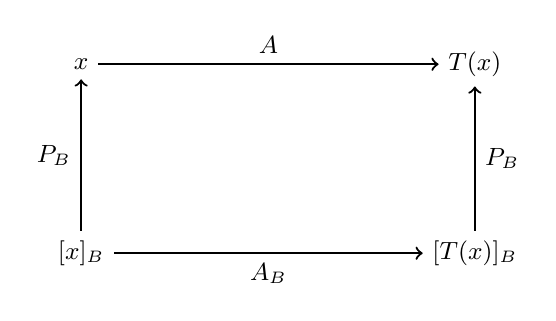
\begin{tikzpicture}[scale=1.0, every node/.style={font=\small}]
    \node (leftbottom) at (0,0) {$[x]_B$};
    \node (rightbottom) at (5,0) {$[T(x)]_B$};
    \node (lefttop) at (0,2.4) {$x$};
    \node (righttop) at (5,2.4) {$T(x)$};
    \draw[->, thick] (leftbottom) -- node[below] {$A_B$} (rightbottom);
    \draw[->, thick] (lefttop) -- node[above] {$A$} (righttop);
    \draw[->, thick] (leftbottom) -- node[left] {$P_B$} (lefttop);
    \draw[->, thick] (rightbottom) -- node[right] {$P_B$} (righttop);
  \end{tikzpicture}
  \caption{The same linear map can be described in standard coordinates or in
  $B$-coordinates. The diagram commutes precisely when
  $A_B=P_B^{-1}AP_B$.}
\end{figure}

\section{Similar Matrices}

\begin{definition}[Similarity]
Matrices $A$ and $C$ in $\R^{n\times n}$ are \emph{similar} if there is an
invertible matrix $P$ such that
\[
  C=P^{-1}AP.
\]
\end{definition}

Similar matrices are different coordinate descriptions of the same linear
transformation. They are not usually equal, but they have the same structural
information.

\begin{proposition}[Similarity preserves eigenvalues]
If $C=P^{-1}AP$, then $A$ and $C$ have the same eigenvalues.
\end{proposition}

\begin{proof}
For any scalar $\lambda$,
\[
  C-\lambda I
  =
  P^{-1}AP-\lambda P^{-1}IP
  =
  P^{-1}(A-\lambda I)P.
\]
Thus $C-\lambda I$ is invertible exactly when $A-\lambda I$ is invertible.
So the values of $\lambda$ for which invertibility fails are the same for both
matrices. Those values are the eigenvalues.
\end{proof}

\begin{proposition}[Trace is similarity invariant]
If $C=P^{-1}AP$, then
\[
  \Trace(C)=\Trace(A).
\]
\end{proposition}

\begin{proof}
The trace has the cyclic property $\Trace(XY)=\Trace(YX)$ whenever the products
are defined. Therefore
\[
  \Trace(P^{-1}AP)
  =
  \Trace(APP^{-1})
  =
  \Trace(A).
\]
\end{proof}

\section{A Basis Can Reveal The Mechanism}

Consider
\[
  A=
  \begin{bmatrix}
  3&1\\
  0&2
  \end{bmatrix}.
\]
In the standard basis, the first coordinate affects the second only indirectly
through the upper-right entry. But if we find a basis of eigenvectors, the same
map becomes diagonal.

For this matrix,
\[
  \lambda_1=3,\qquad \lambda_2=2.
\]
Eigenvectors may be chosen as
\[
  v_1=\begin{bmatrix}1\\0\end{bmatrix},
  \qquad
  v_2=\begin{bmatrix}-1\\1\end{bmatrix}.
\]
Let
\[
  P=\begin{bmatrix}1&-1\\0&1\end{bmatrix}.
\]
Then
\[
  P^{-1}AP=
  \begin{bmatrix}
  3&0\\
  0&2
  \end{bmatrix}.
\]
In the eigenbasis, the transformation simply stretches one coordinate by $3$
and the other by $2$.

\begin{aimlbox}
Basis choice is an interpretability tool. In data settings, a useful basis can
separate directions of variation, decouple coordinates, or expose independent
modes. The spectral chapters will make this precise for symmetric matrices and
for SVD.
\end{aimlbox}

\section{Matrix Powers}

Similarity is also computationally useful. If
\[
  A=PDP^{-1},
\]
where $D$ is diagonal, then
\[
  A^k = PD^kP^{-1}.
\]
Powers of diagonal matrices are easy:
\[
  D=
  \begin{bmatrix}
  \lambda_1&0\\
  0&\lambda_2
  \end{bmatrix}
  \quad\Longrightarrow\quad
  D^k=
  \begin{bmatrix}
  \lambda_1^k&0\\
  0&\lambda_2^k
  \end{bmatrix}.
\]
This is the algebra behind many discrete-time systems:
\[
  x_{k+1}=Ax_k,\qquad x_k=A^kx_0.
\]

\section{Python Thread}

\begin{lstlisting}
import numpy as np

A = np.array([[3.0, 1.0],
              [0.0, 2.0]])

P = np.array([[1.0, -1.0],
              [0.0,  1.0]])

A_B = np.linalg.solve(P, A @ P)   # P^{-1} A P, without forming P^{-1}
print(A_B)

x_B = np.array([2.0, -1.0])
x_standard = P @ x_B

left = A @ x_standard
right = P @ (A_B @ x_B)
print(np.allclose(left, right))

k = 8
D_power = np.diag(np.diag(A_B)**k)
A_power_from_basis = P @ D_power @ np.linalg.solve(P, np.eye(2))
print(np.allclose(A_power_from_basis, np.linalg.matrix_power(A, k)))
\end{lstlisting}

\begin{labbox}
Lab 8 practices coordinate conversion, similarity, and diagonalization in
small matrices. The goal is not to memorize formulas; it is to keep track of
which coordinate system each vector lives in.
\end{labbox}

\section*{Chapter Summary}
\addcontentsline{toc}{section}{Chapter Summary}

\begin{itemize}
  \item A vector is independent of coordinates, but its coordinate list depends
        on the chosen basis.
  \item If $P_B$ has basis vectors as columns, then $v=P_B[v]_B$ and
        $[v]_B=P_B^{-1}v$.
  \item The matrix of a linear map in basis $B$ is $A_B=P_B^{-1}AP_B$.
  \item Similar matrices describe the same linear map in different bases.
  \item A good basis can simplify a transformation and prepare the way for
        diagonalization, spectral theory, and SVD.
\end{itemize}

\section*{Exercises}
\addcontentsline{toc}{section}{Exercises}
\subsection*{A. Theory}
\begin{exercise}\exerciseid{10.A1} Prove the Cauchy-Schwarz inequality in the special case of $\R^2$ using the discriminant method. \end{exercise}
\subsection*{B. By Hand}
\begin{exercise}\exerciseid{10.B1} Project $v=(3,4)$ onto the line spanned by $u=(1,1)$. \end{exercise}
\subsection*{C. Python / NumPy}
\begin{exercise}\exerciseid{10.C1} Write a function that computes cosine similarity between two nonzero vectors. \end{exercise}
\subsection*{D. Challenge}
\begin{exercise}\exerciseid{10.D1} Give two different inner products on $\R^2$ for which the same two vectors have different angles. \end{exercise}

